% % % % % % % % % % % % % % % % % % % % % % % % % % % % % % % % % % % % % % % % %
% INTRO
% % % % % % % % % % % % % % % % % % % % % % % % % % % % % % % % % % % % % % % % %
\section{Time box 6}
\listoftodos
\subsection{Time box planning}

\begin{figure}[H]
	\begin{centering}
		\missingfigure{Updated timebox figure}
		%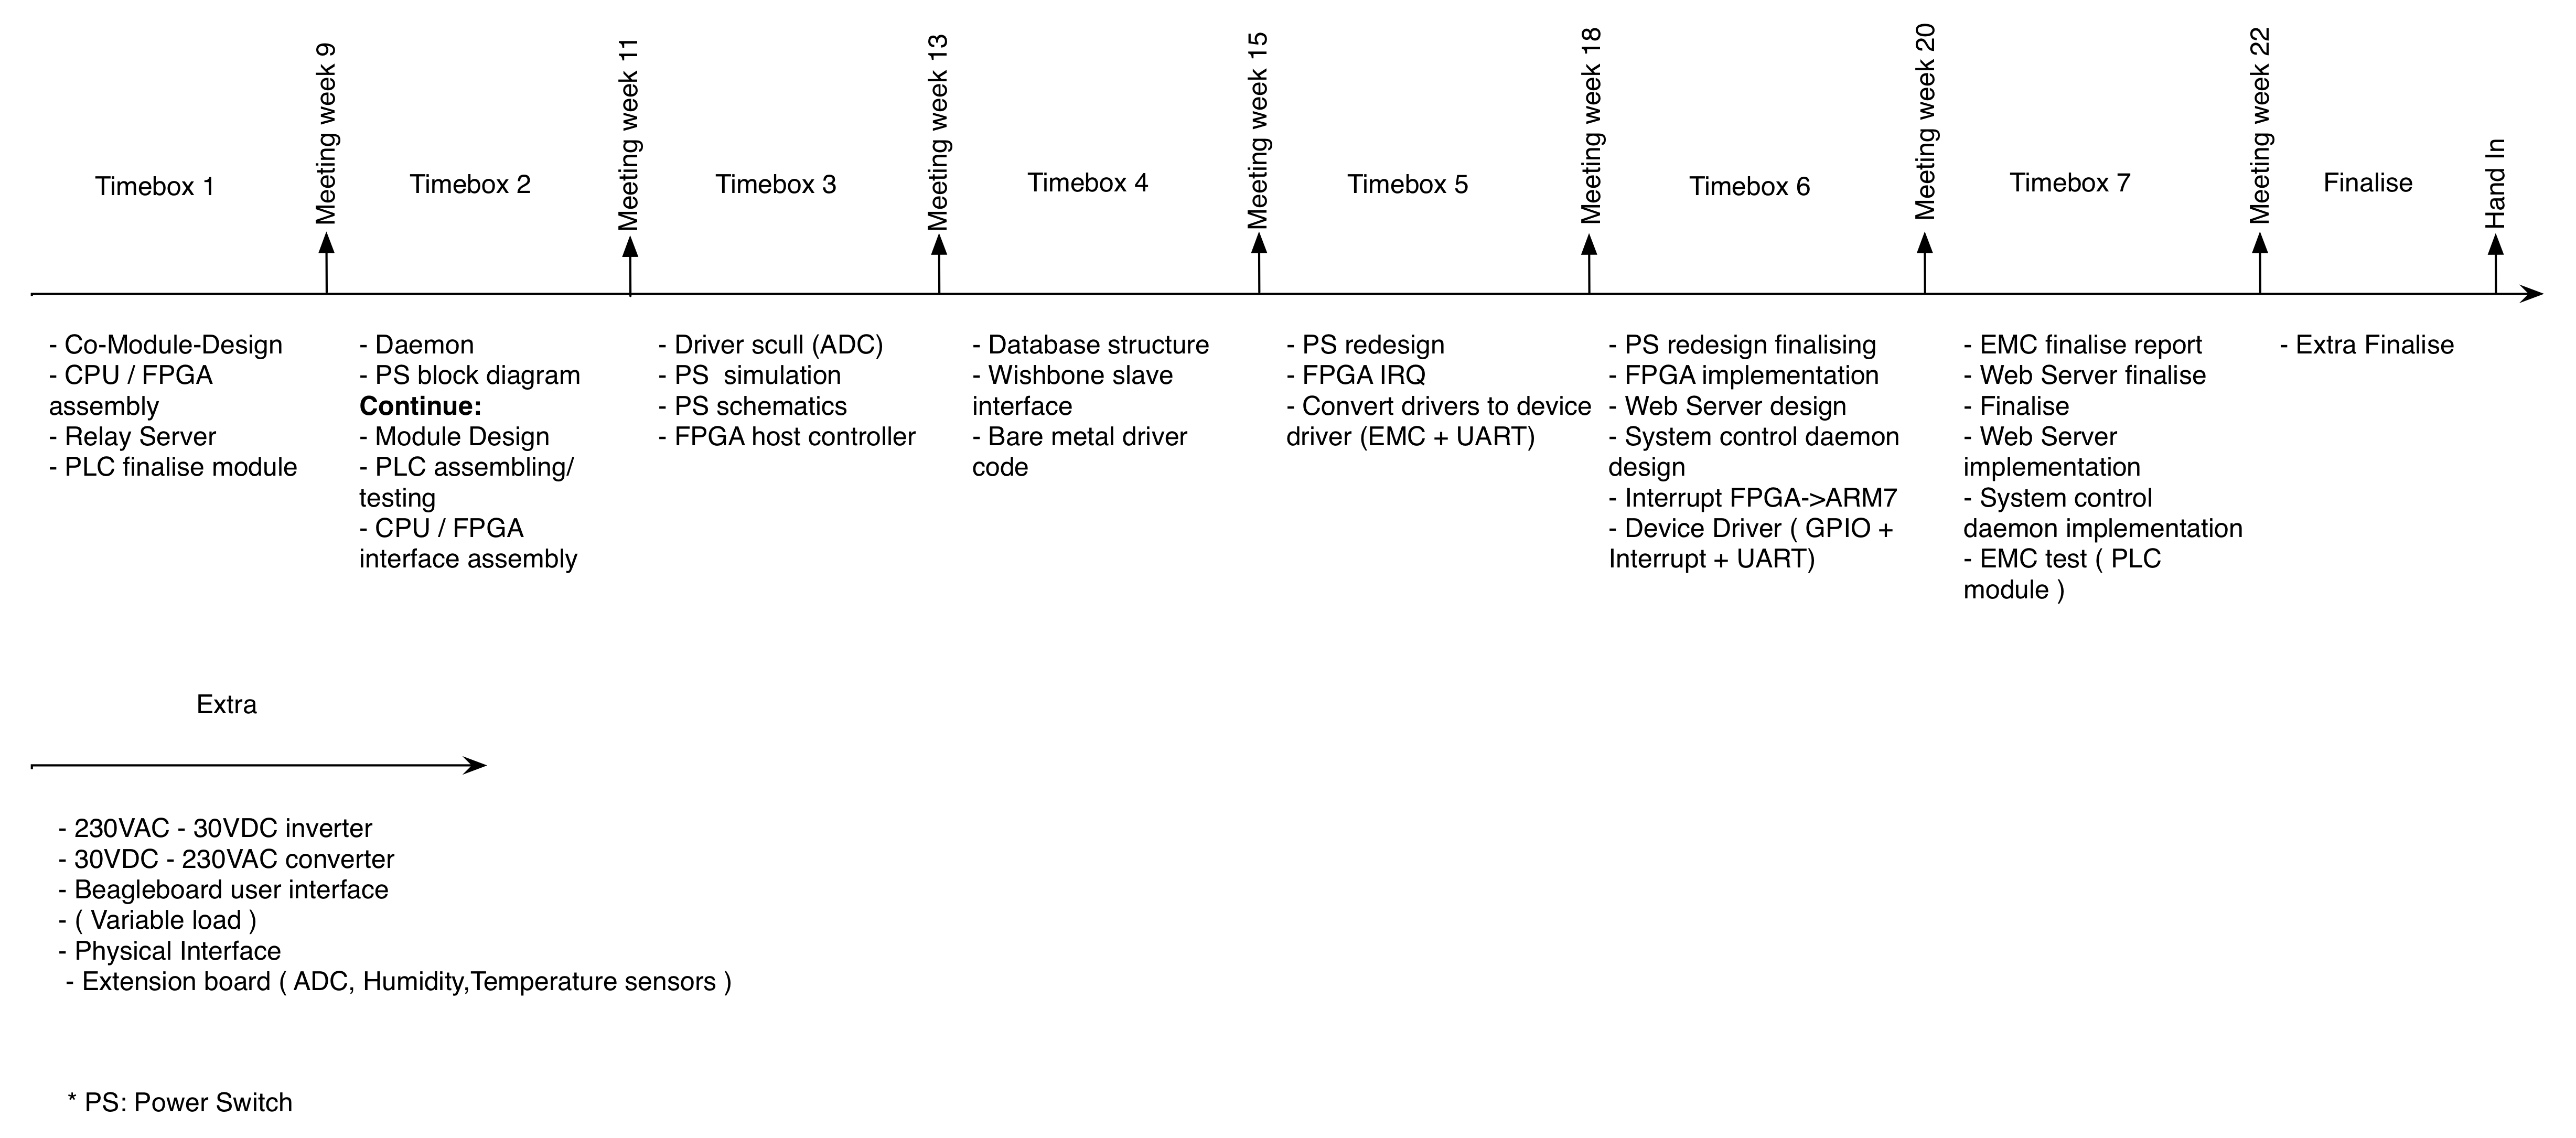
\includegraphics[width=1.0\textwidth]{images/tb_r5.png}
		%\caption{Updated time-box}
	\end{centering}
\end{figure}

\subsubsection{Work to be done in this time box}
\todo[inline]{Update List}
\begin{itemize}
	\item Switch interrupt
	\begin{itemize}
		\item debouncer
		\item Interrupt
	\end{itemize}
	\item Jesus thing
		\begin{itemize}
			\item sub thing
		\end{itemize}
	\item UART Device driver
	\begin{itemize}
		\item Improvement on the driver made in last timebox
	\end{itemize}
\end{itemize}

\paragraph{Description:}
\todo[inline]{Update Description}
\begin{description}
	\item[Switch interrupt] In order to send data to the interrupt register, an interrupt output for the switch block has to be implemented, and the switches has to be debounced, to secure that the interrupt data is send only once.
	\item[Jesus thing]
	\item[UART Device driver] Implementation of input/output control and interrupt handling in the UART device driver made in time box 5.
\end{description}

\subsubsection{Time planning}

\begin{table}[H]
\centering
	\todo[inline]{Update Time}
	\begin{tabular}{|l|c|c|c|c|c|}
		\hline
		~			& Switch interrupt		& Jesus thing		& UART improvements	\\ \hline
		Estimation	& 12					& xx				& 5					\\
		Actual		& 20					& xx				& 15					\\
		Developer	& Theis				& Paulo			& Dennis				\\
		\hline
	\end{tabular}
	\caption{Estimation and actual time used on the project}
\end{table}

% % % % % % % % % % % % % % % % % % % % % % % % % % % % % % % % % % % % % % % % %
% % % % % % % % % % % % % % % % % % % % % % % % % % % % % % % % % % % % % % % % %
% Scaling the project due to limited time.
% % % % % % % % % % % % % % % % % % % % % % % % % % % % % % % % % % % % % % % % %
\subsection{Project scaling}
Unfortunately there is still a lot of work tasks to be done before the fully project is realized. With only 2 weeks before delivering the report it has been decided to down scale the project, to have some blocks fully up and running. The picture below shows the parts that will hopefully be implemented in the handed in version. 
\begin{figure}[H]
	\begin{centering}
		%\missingfigure{Updated timebox figure}
		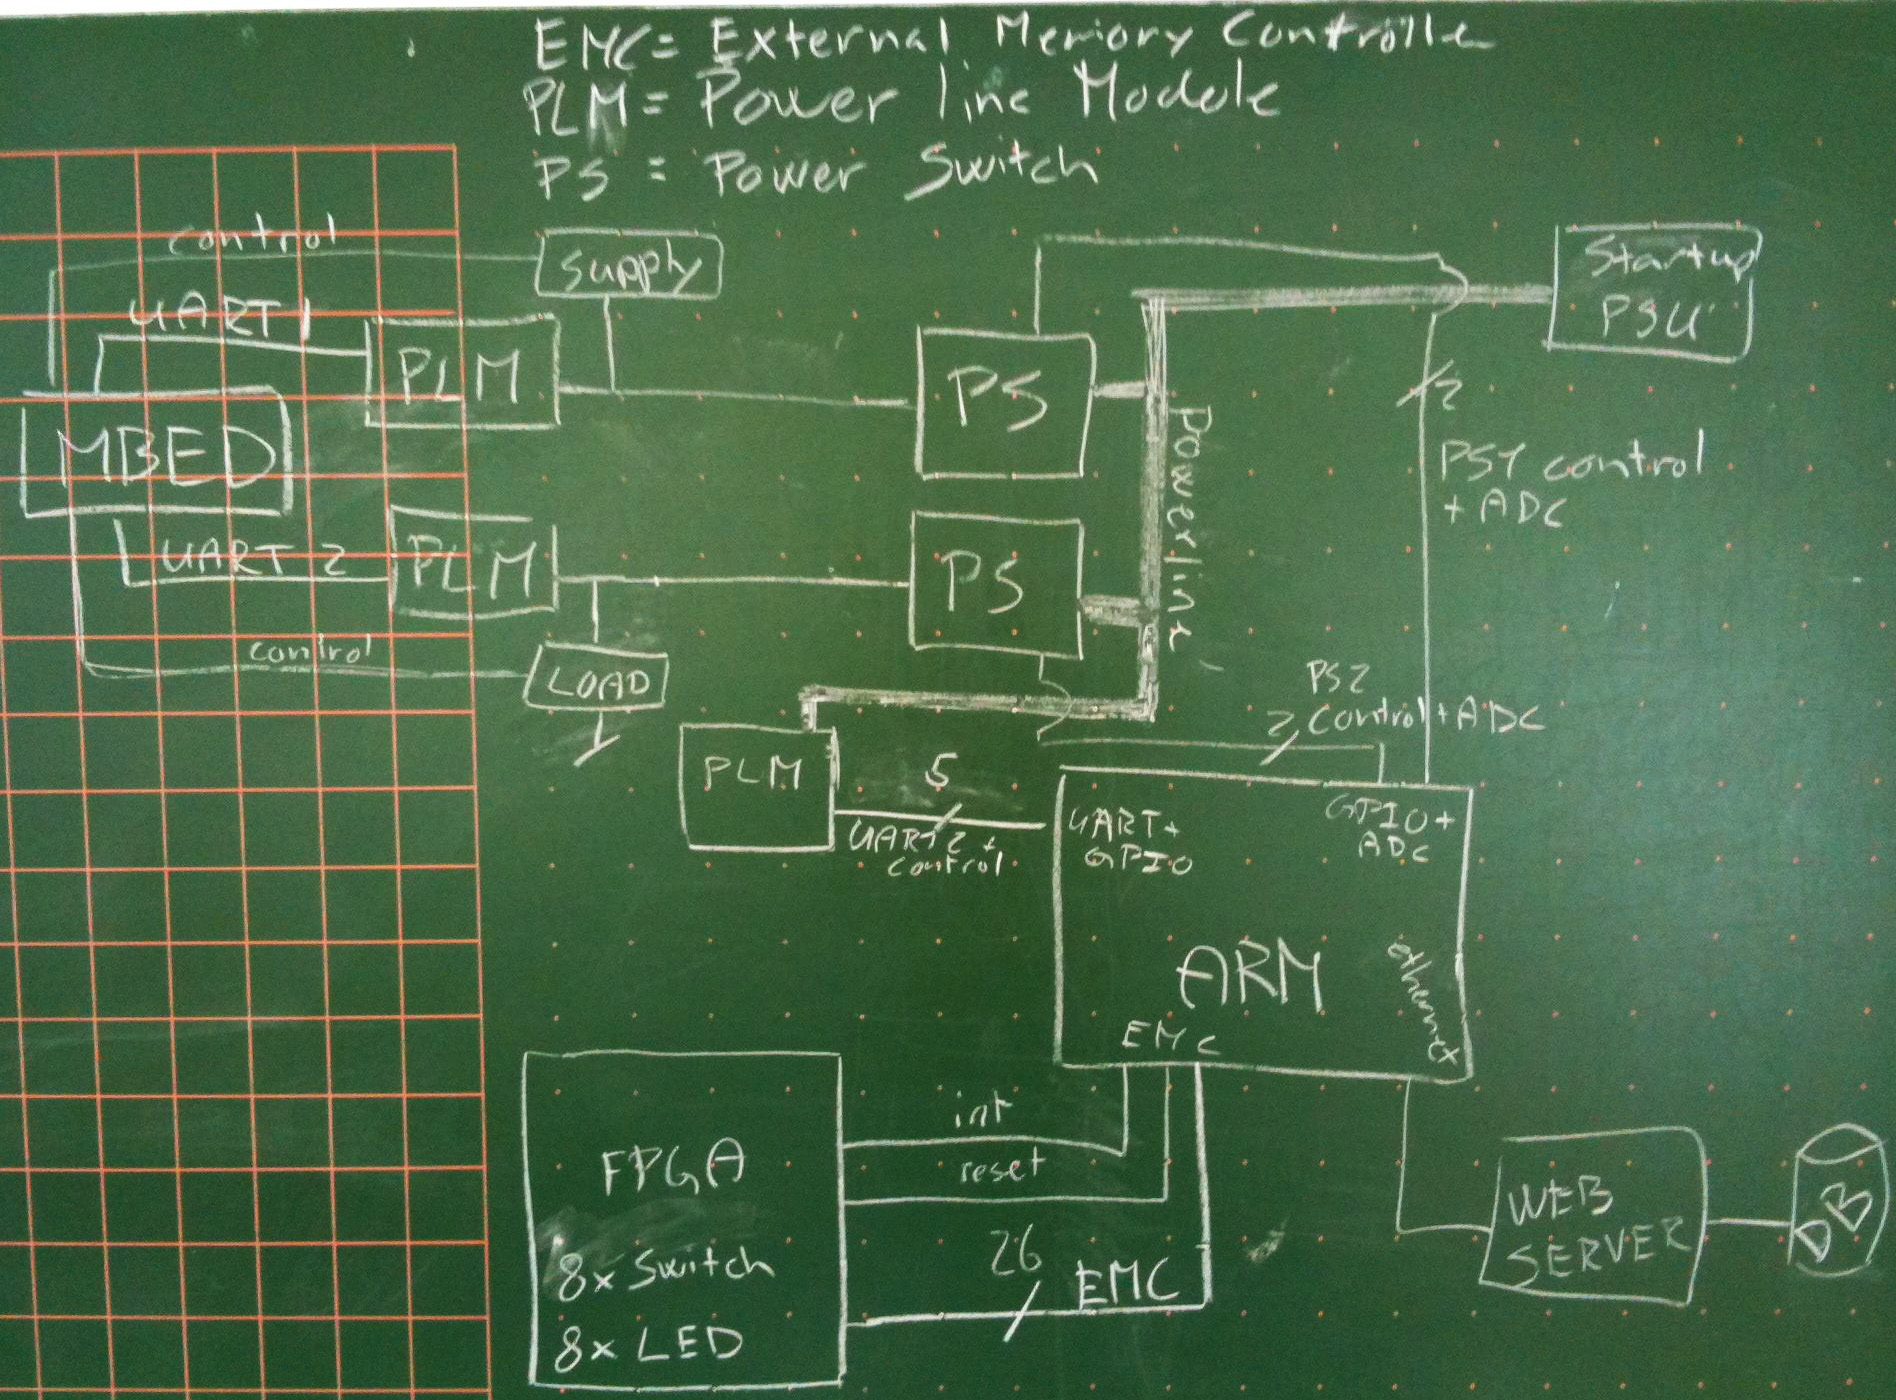
\includegraphics[width=1.0\textwidth]{images/project_scaling_tb6.jpg}
		\caption{Project Scaling diagram}
	\end{centering}
\end{figure}
\textbf{The scaled project will then contain:} 
\begin{itemize}
	\item ARM to FPGA communication through External Memory Controller. The ARM gets an interrupt from the FPGA whenever a switch changes status. The ARM then sets the LEDS on the ARM board according to the switches status.
	\item UART communication to Power Line Module to send and transmit data between two modules. 
	\item MBED setup to work as two modules (communicating with the ARM board through two power line modules).
	\item Dummy protocol to send data from MBED to ARM board. 
	\item Direct received data from MBED to WEB-server.
	\item \todo[inline]{JESUS, something about database and web server}
	\item ...
\end{itemize} 
The setup will then be able to check which state it should be running in, according to the switches set on the FPGA board. The ARM board will be able to control the Power Line modules (switching direction and turning off modules). When communication is established between the MBED and the ARM through Power Line, the data received from the MBED is verified and sent to the WEB-server. 
\todo[inline]{JESUS, something about database and web server}

% % % % % % % % % % % % % % % % % % % % % % % % % % % % % % % % % % % % % % % % %
% % % % % % % % % % % % % % % % % % % % % % % % % % % % % % % % % % % % % % % % %
% Theis Thing
% % % % % % % % % % % % % % % % % % % % % % % % % % % % % % % % % % % % % % % % %
\subsection{Switch interrupt - Theis}
%			Intro
%					verification specification
%					deployment specification
%
This part is, together with the interrupt register from earlier timebox a way to tune performance in reading and writing between the Spartan 6 and the LPC2478.
\subsubsection{Analysis}
%			Analysis
%
%                Refactored block diagram
%                Refactored class diagram
%                Detailed use cases
%                User interface specification
%                System interface specification
%                Dimensioning specification 
%
The interrupt block in the Spartan 6 is the switch block. The switch block needs to be redesign in order to get an interrupt output to the interrupt register, the switches also needs to be debounced, to prevent it from sending the same interrupt data more than once. Two output is added to the switch block, one single bit for interrupt indication and a 7 bit vector for the data to the interrupt register. Inside the block a finite state machine is made for denouncing the switches. Below the redesigned switch block is shown.

\begin{figure}[H]
	\begin{centering}
		%\missingfigure{Updated timebox figure}
		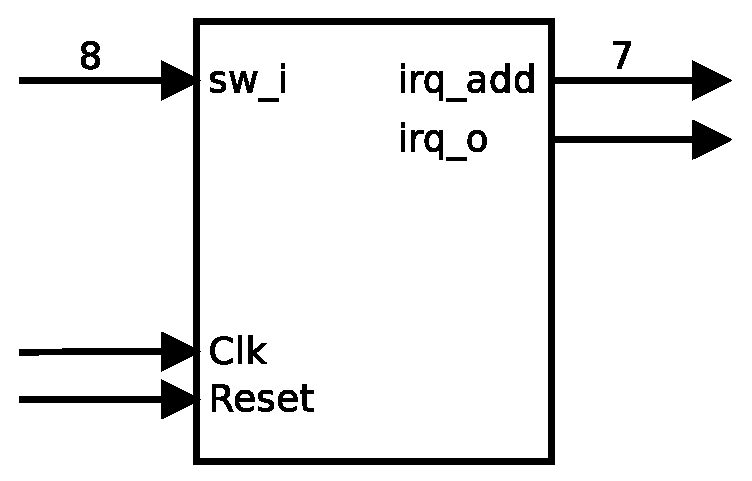
\includegraphics[width=0.3\textwidth]{images/tb6_switchblock.eps}
		\caption{Updated switch block}
	\end{centering}
\end{figure}


\subsubsection{Design}
%       	 Design
%
%                UML/SysML deployment view(s)
%                Mechanical specifications and dimensioning
%                HW module specification per block
%                UML SW deployment view
%                Class specification
%                Refactored class diagram
%                Use case scenarios specifications
%                Sequence diagrams
%
Because of switch bounce, the block needs to take care of this. Below a picture of switch bouncing is shown. The problem is every time the signal goes high the switch block will send data to the interrupt register, to prevent this the block compare a delayed input signal to the present signal, and first when the signal is stable, the system will react on the input.

\begin{figure}[H]
	\begin{centering}
		%\missingfigure{Updated timebox figure}
		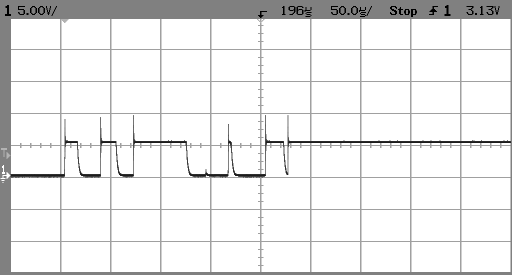
\includegraphics[width=0.5\textwidth]{images/tb6_bounce.png}
		\caption{Switch bouncing}
	\end{centering}
\end{figure}

To debounce the switch a state machine for the switch block is made. This diagram is shown below. The start box set the start output signal to the input signal. The interrupt signal is set high in the OUT0 state, and low again in the IDLE state after the "q2" delay. This is done to have the interrupt signal high enough time for the interrupt register to save the data. The "q1" delay is used to compare the input signal with the output signal in order to capture changes on the 8 switches.

\begin{figure}[H]
	\begin{centering}
		%\missingfigure{Updated timebox figure}
		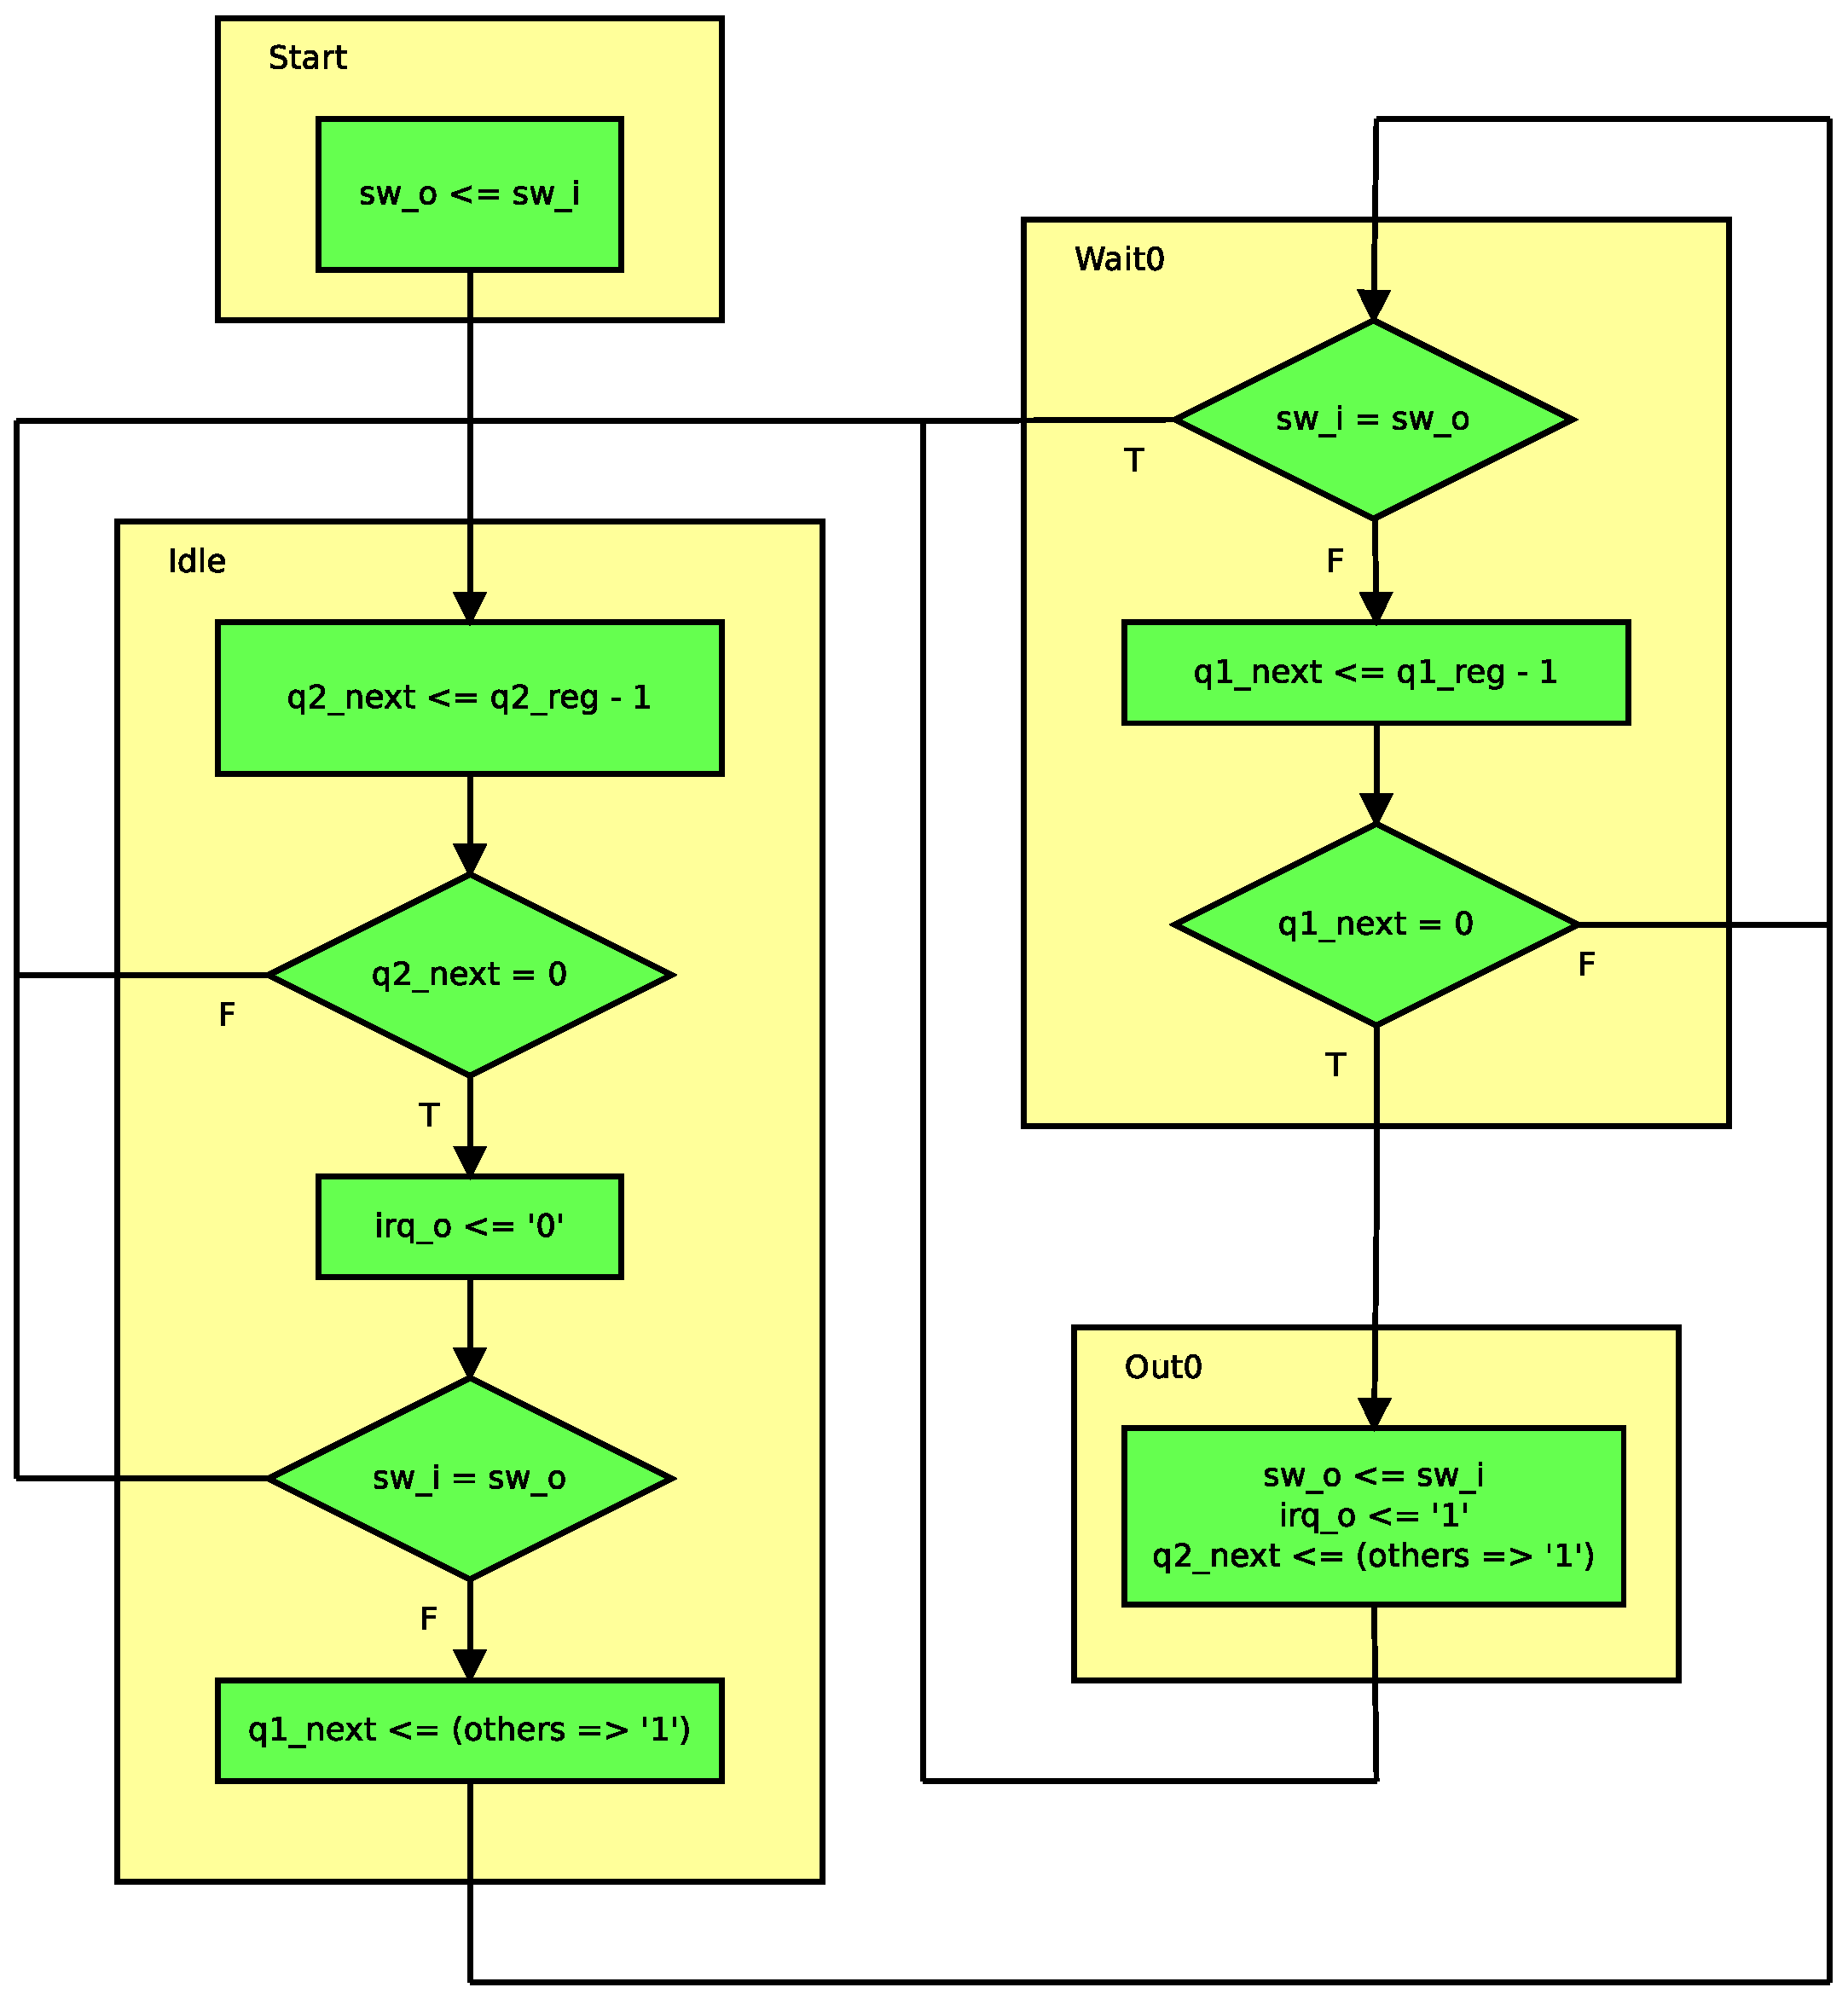
\includegraphics[width=0.7\textwidth]{images/tb6_switch_FSD.eps}
		\caption{Switch block state machine}
	\end{centering}
\end{figure}

\subsubsection{Implementation}
%     	   Implementation
%
%                Mechanical drawings with details explained
%                Electronic diagrams with details explained
%                Source code with details explained
%                Description of integration 
%
The code for the IDLE state is shown below, here the "q2" delay is used in the start, then the interrupt pin is set to zero, then the input and output is compared, if they are not equal the next state is WAIT0 and the "q1" delay is set.
\begin{lstlisting}[language=VHDL]
...
when IDLE =>
	q2_next <= q2_reg-1;
	if	(q2_next = 0) then
		irq_o <= '0';
		if	(sw_i = sw_o) then
			state_next <= IDLE;
		else
			q1_next		<= (others => '1');
			state_next	<= WAIT0;
		end if;
	else
		state_next <= IDLE;
	end if;
...
\end{lstlisting}
In the WAIT0 state the input and output is compared repeatedly to check if the input is stable. If the input is stable long enough time the OUT0 state is entered.
\begin{lstlisting}[language=VHDL]
...
when WAIT0 =>
	if	(sw_i = sw_o) then
		state_next <= IDLE;
	else
		q1_next <= q1_reg-1;
		if	(q1_next = 0) then
			state_next <= OUT0;
		else
			state_next <= WAIT0;
		end if;
	end if;
...
\end{lstlisting}
In the OUT0 state the switch output is set to switch input signal, and an interrupt signal is set high, the "q2" delay is set and it returns to the IDLE state.
\begin{lstlisting}[language=VHDL]
...
when OUT0 =>
	sw_o		<= sw_i;
	irq_o		<= '1';
	q2_next		<= (others => '1');
	state_next	<= IDLE;
...
\end{lstlisting}

\subsubsection{Verification}
%       	 Verification
%
%                Module tests
%                Integration tests
%                Acceptance test
The code is tested on a test bench in isim. The test verify that the block first set the switch output after the input has been stable for a while. And when the output is set the interrupt signal is set high for some time and then set low again. 
\begin{figure}[H]
	\begin{centering}
		%\missingfigure{Updated timebox figure}
		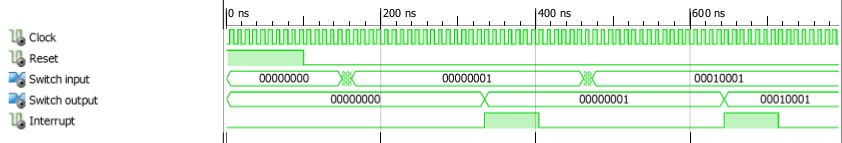
\includegraphics[width=1.0\textwidth]{images/tb6_switch_tb.png}
		\caption{Switch block test bench}
	\end{centering}
\end{figure}
\subsubsection{Conclusion}
The test shows that the interrupt function is working properly, the design is also tested on the Spartan 6 with the LCP2478, and it is working as expected.
% % % % % % % % % % % % % % % % % % % % % % % % % % % % % % % % % % % % % % % % %
% % % % % % % % % % % % % % % % % % % % % % % % % % % % % % % % % % % % % % % % %
% Jesus Thing
% % % % % % % % % % % % % % % % % % % % % % % % % % % % % % % % % % % % % % % % %
\subsection{Web Server - Paulo}
%			Intro
%					verification specification
%					deployment specification
%
In time box 4 a web server was implemented at the ip address 10.1.18.223, this is a virtual machine assign as development environment for the uClinux distribution. The server is running Apache 2, PHP version 5.1.6 and MySQL server 5.0.95.
In this time box a web services system is developed for the communication between the Embedded device and the web server and the other way around. The web page made in Project 3 is incorporated with server side scripts (PHP) for a fully functional web interface.\\
\A user with read only permissions was created:

User: eval

Pass: ede10eval\\

For evaluation reasons a web application is developed with the name SeeIt, this is a PHP web application that allows the user to see the file structure of the server and the file content, this can be seen at http://10.1.18.223/Seeit/.\\
\\The development of the energy hub web interface can be followed at:

http://e10.ede.hih.au.dk/index.php/Web\_Server\_Structure

The database structure for this project was change to a common database to all modules, the new structure can be seen at:

http://e10.ede.hih.au.dk/index.php/Common\_Database

With the credentials above, the user is able to login into the phpMyAdmin tool in the AU-Herning network at the address: http://10.1.18.223/phpMyAdmin where the database structure is implemented.\\

\subsubsection{Analysis}
%			Analysis
%
%                Refactored block diagram
%                Refactored class diagram
%                Detailed use cases
%                User interface specification
%                System interface specification
%                Dimensioning specification 
%
For a fully functional web interface the communication have to present in both direction, since some teams need to send commands from them web page to the modules.
A file structure was created in the server, where each team have is own folder where all the needed scripts, images and layout styles can be implemented without changing the common layout and requirements approved in project 3.

In this time box the follow scripts are created:
\begin{itemize}
	\item index.php
	\item savedata.php
	\item sendcmd.php
	\item saveip.php
%	\item ajax.js
%	\item login.php
%	\item cron.php
	\item db\_connect.php
	\item db\_globals.php
\end{itemize}

\paragraph{Web interface file Structure}
The file structure is still in development, as such and for the correct version the structure is updated at the address: 

http://e10.ede.hih.au.dk/index.php/Web\_Server\_Structure
%
A short description for each script can be seen bellow:
\begin{itemize}
	\item index.php - First page of the web interface.
	\item savedata.php - Webservice that save data retrieved from the module to the database.
	\item sendcmd.php - Webservice to send commands to the desired module in the system.
	\item saveip.php - Webservice necessary to save the ip address of the energy hub, this will keep the system up and running even if a change on the network is made.
%	\item ajax.js - This Javascript handle AJAX requests when the page have no need to be reloaded, that ensure less bandwidth in the web server.
%	\item login.php  - This PHP script makes the authentication of the user, creating a session when the user gives the right certifications.
%	\item cron.php  - Cron jobs are running by the server in a predefined time, in this case the cron.php at the web server root will point to the cron jobs inside each module folder.
	\item db\_connect.php - Handle the connection to the MySQL database.
	\item db\_globals.php - Includes all the global variables with the credentials for the database.
\end{itemize}

\lineparagraph{Communication}
The server have to save the data retrieved from the system and send commands to the modules connected to the energy hub. Two main scripts are created: \textit{savedata.php} this script capture the values send by the HTTP request has a POST method saving them to the database and \textit{sendcmd.php} enables the user to send commands to a precise module in the system or even the energy hub.
\newpage
Measurements to be saved in the database:
\begin{figure}[H]
	\begin{centering}
		%\missingfigure{Communication savedata.php}
		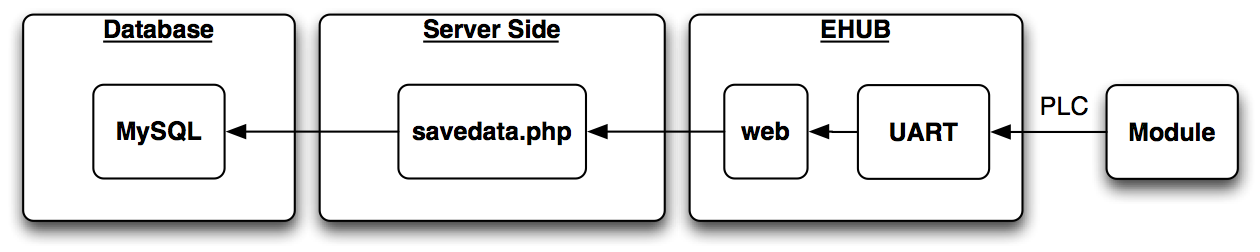
\includegraphics[width=1\textwidth]{images/tb6_webserver_savedata.png}
		\caption{Save measurements retrieved by the modules}
	\end{centering}
\end{figure}
To retrieve the measurements from the modules, an application running at the energy hub translate the data retrieved from the module through PLC to a URL request at the web server. In the server side the web server will collect the data and save it in the database.

Flow of the communication from the user until the final destination in this case the module or the energy hub.
\begin{figure}[H]
	\begin{centering}
		%\missingfigure{Communication SendCmd.php}
		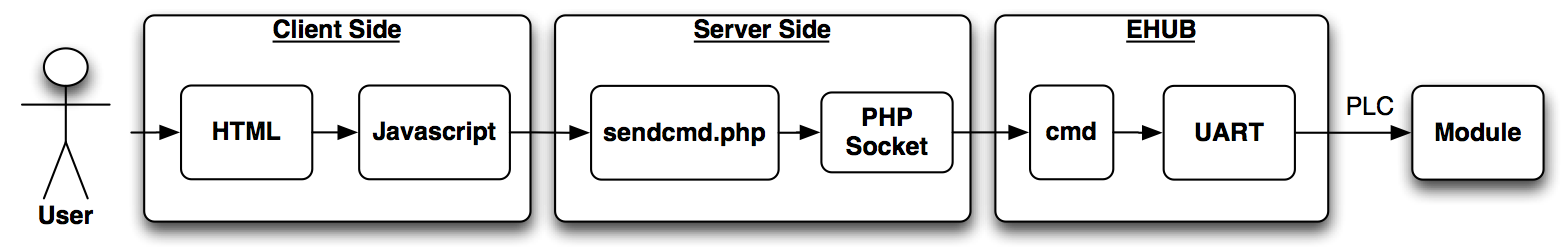
\includegraphics[width=1\textwidth]{images/tb6_webserver_sendcmd.png}
		\caption{Send a command to a module}
	\end{centering}
\end{figure}
This script doesn't give a feedback to the user, the commands send are not verified by the web server or the energy hub. The commands are handle by each module. With this system the flexibility of the system is ensured, since new modules can be added with different functionalities from the already known.
An application running in background at the energy hub OS, ensure that the command is translated to UART so it can be send through the power line communication to the modules.
\\

IP address is send from the Embedded Device:
\begin{figure}[H]
	\begin{centering}
		%\missingfigure{Communication SendCmd.php}
		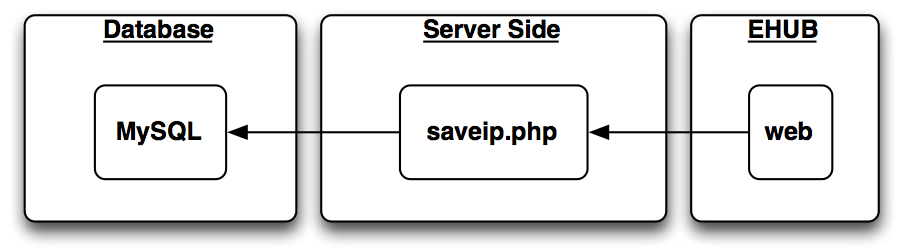
\includegraphics[width=0.8\textwidth]{images/tb6_webserver_saveip.png}
		\caption{Save the IP address of the Embedded device}
	\end{centering}
\end{figure}
A background application running (daemon), ensure that after a reboot, the IP address assigned by DHCP to the energy hub is saved in the database so commands can be send through the web interface. This add flexibility to the system, since a change in the internal network could stop the normal work of the system.

\lineparagraph{Structure Generals}

A folder is created for each team, it will contain the necessary scripts to show data for the users, send commands to the energy hub, make their own layout, etc.

This is a necessary structure for this project, since the requirements are different for all the teams. For example the energy hub page needs to show completely different data from the wind turbine or other modules.

In real production software a general layout and data should be set for all the modules pages, being possible to make small adjustments to satisfy the final user/client. This way the final software would have a improved user experience since the layout is equal in all the modules.

\subsubsection{Design}
%       	 Design
%
%                UML/SysML deployment view(s)
%                Mechanical specifications and dimensioning
%                HW module specification per block
%                UML SW deployment view
%                Class specification
%                Refactored class diagram
%                Use case scenarios specifications
%                Sequence diagrams
The main structure for the correct work of the system is created, in the next time box the energy hub page is built to allow the user to stop and start modules, get the current efficiency as green energy system, etc.

\subsubsection{Implementation}
%     	   Implementation
%
%                Mechanical drawings with details explained
%                Electronic diagrams with details explained
%                Source code with details explained
%                Description of integration 
%
\lineparagraph{index.php}

The \textit{index.php} is the main page of the system, this will redirect the users to the modules or login page.
The efficiency of the system can be seen on the first page as the amount of lamps able to power, the money saved and the mount of less CO2 emissions, this is not available in this version, will be part of the hub web page development in next time box.

\lineparagraph{savedata.php}

A background application running in the energy hub converts the measurement sent through PLC (UART) to a HTTP request \textbf{savedata.php?sensor\_id=ID Sensor\&value=Sensor Measurement\&hub\_port=Hub Port}.

\begin{lstlisting}[language=php]
<?php
	
	require_once("db_connect.php");
	
	$date = getdate();
	
	$today = $date['year'].'-'.$date['mon'].'-'.$date['mday'].' '.$date['hours'].':'.$date['minutes'].':'.$date['seconds'];

	if(isset($_GET['sensor_id']) && isset($_GET['value']) && isset($_GET['hub_port'])){
		$sql= "INSERT INTO `iEnergy`.`MEASUREMENTS` (".
			  "`ID_MEASURE` ,".
			  "`ID_SENSOR` ,".
			  "`DATE_TIME` ,".
			  "`HUB_PORT` ,".
			  "`VALUE`)".
			  "VALUES (NULL , '".$_GET['sensor_id']."', '".$today."', '".$_GET['hub_port']."', '".$_GET['value']."')";
	
		$con->query($sql); // Run the query in the MySQL server
		
		// No feedback needed since the energy hub will not expect an answer.
		
	} else {
		echo 'Incorrect parameters';
	}
	
?>
\end{lstlisting}

This script saves the measurement retrieved from a sensor to the database. At first it established the connection to the MySQL server so SQL requests can be made.
A PHP function returns an array with the current date and time, this is formatted into YYYY-M-D H:M:S, after it can be saved to the MEASUREMENTS table. The script collects all the parameters send through the URL encoding GET, a SQL code is generated and a request made to the MySQL server, the data is added to the MEASUREMENTS table.

\lineparagraph{sendcmd.php}

The web interface is able to send commands to the energy hub and the modules using the\\ \textbf{sendcmd.php?id\_module=\textless module id\textgreater\&cmd=\textless command to be send\textgreater }. The id\_module tells the hub which module the command should be send.
No verification is made of the send command by the web server or the energy hub unless the command is specifically send to the hub.

\begin{lstlisting}[language=php]

	// SQL request for the device page.
	require_once("includes/db_connect.php");
	
	if(isset($_GET['cmd']) && isset($_GET['id_module'])){
	
		$device_port = 5555;
		
		//echo 'Module Id: '.$_GET['id_module']."<BR>Command: ".$_GET['cmd']."<BR>";
		
		$sql= "SELECT IP ". 
			  "FROM `DEVICE` ". 
			  "ORDER BY ID_DEVICE DESC ".
			  "LIMIT 1";
		
		$res = $con->query($sql); // Run the query in the MySQL server
		
		$row = $res->fetch_row();
		
		$device_ip = $row[0];
		
		if ($socket=socket_create(AF_INET, SOCK_STREAM, SOL_TCP)){
			echo "Socket created <br>";
		}
	
		if (socket_connect($socket,$device_ip,$device_port)){
			echo "Connection stablished<br>";	
		} else {
			exit (socket_strerror(socket_last_error()));
		}
	
		$str = $_GET['cmd'].';'.$_GET['id_module'];
		
		socket_write($socket,$str);
	
		socket_close($socket);
		
	} else {
		echo 'Command or Module Id not set';
	}
\end{lstlisting}

At first the script will get the ip address of the energy hub, running a SQL code that retrieves the last IP address added to the table DEVICE. With the energy hub ip and a predefined port, a connection is created using a TCP socket for the communication. The command and the module id are send and the socket is closed.

\lineparagraph{saveip.php}

\textit{saveip.php} script is called by the background application running on the embedded device, it saves the IP address given by DHCP, this is used for further communication between the web server and the energy hub.
\begin{lstlisting}[language=php]
	require_once("includes/db_connect.php");

	if(isset($_GET['ip'])){
		$sql= "INSERT INTO `iEnergy`.`DEVICE` (".
			  "`ID_DEVICE` ,".
		  	  "`IP`)".
		  	  "VALUES (NULL , '".$_GET['ip']."')";
	
		$con->query($sql); // Run the query in the MySQL server
		
		// No feedback needed since the energy hub will not expect an answer.
		
	} else {
		echo 'IP not set';
	}
\end{lstlisting}
The ip address is send by the GET method (saveip.php?ip=127.0.0.1), this is how the data in encoded into a URL, being collected in the variable \$\_GET['ip']. 
A \$sql variable string is created containing the SQL code to be run at the MySQL server.

\lineparagraph{db\_connect.php}

For the communication to the database a driver is used in PHP that provides an interface to the MySQL server. The PHP mysqli extension (MySQL improved) is used in this project, this is recommend for MySQL servers version 4.1.3 or later. This extension provides several benefits as a objective-oriented interface, support for multiple statements, embedded server support and more can be found in the MySQL documentation.

\begin{lstlisting}[language=php]
	require_once("db_globals.php");
	
	$con = new mysqli(DB_HOST,DB_USER,DB_PASS,DB_NAME); // Creates new mysql connection
	
	if($con->connect_error){
		echo "Failed to connect to MySQL: (" . $con->connect_errno . " ) ". $con->connect_error;
	} 
	else { echo "Connection established"; }
\end{lstlisting}

In this script an object is instantiated with a connection to the MySQL server.

\textit{\$con = new mysqli\textless parameters \textgreater)}

The parameters are included from the db\_globals.php, setting the server host, user, password and database to be used.

\lineparagraph{db\_globals.php}

Using a script to define the parameters for the MySQL connection, 
All the scripts that need to use the global parameters for the connection to the MySQL server, should include db\_globals.php as shown in the db\_connect.php above.

\begin{lstlisting}[language=php]
	// MySQL condifuration
	DEFINE ('DB_USER','root');
	DEFINE ('DB_PASS','root');
	DEFINE ('DB_HOST','localhost');
	DEFINE ('DB_NAME','iEnergy');
\end{lstlisting}

The global parameters the connection to the MySQL server are define in this script.

\begin{itemize}
	\item DB\_USER - Database user name with read, write and execute permissions.
	\item DB\_PASS - Password for the user
	\item DB\_HOST - Hostname for the MySQL server, if running at the same host as the PHP server, localhost or 127.0.0.1 should be used.
	\item DB\_NAME - Database name to connect to.
\end{itemize}

\subsubsection{Verification}
%       	 Verification
%
%                Module tests
%                Integration tests
%                Acceptance test
The verification is made using the tools described in the beginning of this section:
\begin{table}[H]
\centering
	\begin{tabular}{| c | l | c |}
		\hline
		Verification & Description & Acceptance \\\hline
		1 & Save new IP address: saveip.php?ip=127.0.0.1 & OK \\\hline
		2 & Send command: sendcmd.php?unique\_id=0\&cmd=led 1 on & TimeBox7 \\\hline
		3 & File structure created & OK \\\hline
	\end{tabular}
\end{table}

\subsubsection{Conclusion}
The common web services and file structure in the web server was created for all the modules/teams.\\
The implementation of the savedata.php will required further analysis for a working system, since the energy hub needs to have a table of all the sensors connected to each module. When a module retrieves a value the hub needs to know which sensor the measurement belongs to. This was not taken in consideration in earlier analysis of the system and might affect the protocol developed and system dynamics.\\
In the next time box a scaled down prototype is developed and the communication dynamics between web server and modules can be tested.

% % % % % % % % % % % % % % % % % % % % % % % % % % % % % % % % % % % % % % % % %
% % % % % % % % % % % % % % % % % % % % % % % % % % % % % % % % % % % % % % % % %
% Dennis Thing
% % % % % % % % % % % % % % % % % % % % % % % % % % % % % % % % % % % % % % % % %
\subsection{UART Device driver improvements - Dennis}
As described in section \ref{sec:device_driver_conclusion}, some improvements should be implemented in order to boost performance on the UART devices. The parts which will be further implemented in the UART device driver is:
\begin{itemize}
	\item Interrupt controlled read.
	\item More flexibel initialization. 
	\item Better feedback/help description to the user. 
\end{itemize}
Furthermore it was pointed out (by Klaus Kolle) that the implemented way of setting up the device broke general politic for device drivers. To avoid this, an IOCTL (Input Output Control) function shall be implemented to take care of all setup and to leave the write function to sending characters. 
%			Intro
%					verification specification
%					deployment specification
%
%\subsubsection{Analysis}
%			Analysis
%
%                Refactored block diagram
%                Refactored class diagram
%                Detailed use cases
%                User interface specification
%                System interface specification
%                Dimensioning specification 
%
\subsubsection{Design}
The functionalities implemented in the IOCTL call are:
\begin{itemize}
	\item Help command. Write out the different choices of IOCTL calls.
	\item Default setup call. Sets up the defined UART to 8n1, 9600 baud rate. 
	\item Baud rate. Set a baud rate in the range 2400 to 230400.
	\item Word length. Define the word length between 5 and 8.
	\item Stop bits. Number of stop bits, 1 or 2.
	\item Parity bits. Define parity bit setting: none, odd, even, forced 1 stick, forced 0 stick.
	\item Fifo. Enable or disable fifo.
	\item Fifo trigger. Number of characters in the buffer before an interrupt: 1,4,8,14
\end{itemize}

%       	 Design
%
%                UML/SysML deployment view(s)
%                Mechanical specifications and dimensioning
%                HW module specification per block
%                UML SW deployment view
%                Class specification
%                Refactored class diagram
%                Use case scenarios specifications
%                Sequence diagrams
%
\subsubsection{Implementation}
Common header file for the UART device driver and the UART user space application. The magic number 'k' is used to by the IOCTL macros \_IO and \_IOR to create an IOCTL number, which is then decoded and verified in the kernel module. 
\begin{lstlisting}[language=c]
#ifndef UARTIOCTL_H
#define UARTIOCTL_H

#include <linux/ioctl.h>

#define UART_IOC_MAGIC  'K'

#define IOCTL_HELP 		_IO(UART_IOC_MAGIC,  1)
#define IOCTL_DEFAULT	_IO(UART_IOC_MAGIC,  2)
#define IOCTL_BAUD 		_IOR(UART_IOC_MAGIC, 3, int)
#define IOCTL_WORDLEN 	_IOR(UART_IOC_MAGIC, 4, int)
#define IOCTL_STOPBIT 		_IOR(UART_IOC_MAGIC, 5, int)
#define IOCTL_PARBIT 		_IOR(UART_IOC_MAGIC, 6, int)
#define IOCTL_FIFO			_IOR(UART_IOC_MAGIC, 7, int)
#define IOCTL_FIFO_TRIG 	_IOR(UART_IOC_MAGIC, 8, int)

#define UART_IOC_MAXNR 8

#endif
\end{lstlisting}

Using IOCTL to setup UART registers. Note that the \textit{fwrite} call cannot be used with IOTCL, as it needs an file descriptor instead of a file pointer. Therefore the libraries \textit{fcntl.h} and \textit{unistd.h} are included in order to use the functions \textit{open, close, read, write} and \textit{ioctl} as they make use of the file descriptor. 
\begin{lstlisting}[language=c]
	if(strncmp("io", argv[1], 2) == 0){
		if ((fd = open(UART,O_RDWR)) < 0){
     	          	printf("Cannot open file.\n");
			exit(-1);
        	}

		ret_val = ioctl(fd, IOCTL_DEFAULT);
		if(ret_val < 0){
			printf("ioctl_get_msg failed:%d\n", ret_val);
			exit(-1);
		}
		ret_val = ioctl(fd, IOCTL_BAUD, 19200);
		if(ret_val < 0){
			printf("ioctl_get_msg failed:%d\n", ret_val);
			exit(-1);
		}

		close(fd);
	}
\end{lstlisting}
Loop reading used for testing purpose of the power line communication. 
\begin{lstlisting}[language=c]
	---
	else if(strncmp("readloop", argv[1], 8) == 0){
		if ((fd = open(UART,O_RDONLY)) < 0){		//Open the file
     	          	printf("Cannot open file.\n");
			exit(-1);
        	}
		while(1){
			if(read(fd,rb,10) != 0) 
				printf("%s\n",rb);
		}
		printf("\n");
		close(fd);
	}
\end{lstlisting}

IOCTL added to file operator
\begin{lstlisting}[language=c]
static struct file_operations uart_fops = {
	.owner   	= THIS_MODULE,
	.read			= uart_read,
	.write  	= uart_write,
	.open    	= uart_open,
	.ioctl	 	= uart_ioctl,
	.release 	= uart_close,
};
\end{lstlisting}

IOCTL implementation. At first the function verifies the IOCTL number sent and checks if the transferred command is valid. The rest of the function is a  switch/case which takes the cmd parameter sent and performs an action according to the command (help, default setup, baud rate etc.)
\begin{lstlisting}[language=c]
/******************************************************************************
 * IOCTL call
 *****************************************************************************/
static int uart_ioctl(struct inode *inode, struct file *filp, unsigned int cmd, unsigned long arg){
	unsigned int num = 0;
        int err = 0, ret = 0;
	int div, mult,bflag = 0;
	unsigned int baud = 0;

        /* don't even decode wrong cmds: better returning  ENOTTY than EFAULT */
        if (_IOC_TYPE(cmd) != UART_IOC_MAGIC) return -ENOTTY;
        if (_IOC_NR(cmd) > UART_IOC_MAXNR) return -ENOTTY;

        /*
         * the type is a bitmask, and VERIFY_WRITE catches R/W
         * transfers. Note that the type is user-oriented, while
         * verify_area is kernel-oriented, so the concept of "read" and
         * "write" is reversed
         */
        if (_IOC_DIR(cmd) & _IOC_READ) err = !access_ok(VERIFY_WRITE, (void __user *)arg, _IOC_SIZE(cmd));
        else if (_IOC_DIR(cmd) & _IOC_WRITE) err =  !access_ok(VERIFY_READ, (void __user *)arg, _IOC_SIZE(cmd));
        if (err) return -EFAULT;
	// Get minor number
	num = MINOR(inode->i_rdev);
	DPRINT("\nuart%d_ioctl, ioctl_cmd: %u\n",num,cmd);
	// Check if minor number is okay
	if(num >= NUM_UART_DEVICES){
		return -ENODEV;
	}

	switch (cmd) {
	/***************************** HELP ************************************************/
	case IOCTL_HELP:
	    DPRINT("\nHELP\n");
	    help();	// Print different IOCTL call options to user
	  break;
	/***************************** DEFAULT *********************************************/
	case IOCTL_DEFAULT:
	    m_reg_write(ulcr[num], 0x80);	// Enable write to divisor latch
	    m_reg_write(udll[num], (unsigned char)((LPC24xx_Fpclk/(16*9600)) & 0xFF));
	    m_reg_write(udlm[num], (unsigned char)((LPC24xx_Fpclk/(16*9600)) >> 8));
	    m_reg_write(ulcr[num], 0x03);	// 8N1 setup and disable write to divisor latch
	    m_reg_write(ufcr[num], 0x7);	// Enable FIFO's
	  break;
	/***************************** BAUD ************************************************/
	case IOCTL_BAUD:
	    if(arg < 2400 || arg > 230400){	// Verify argument
		printk("\nInvalid parameter");
		return -EFAULT;
	    }
	    bflag = 0;	
	/* From datasheet:
	   Mult values: 1-15, Div: 0-14. Mult shall be bigger than div.
	   DLL shall be above 2 if DLM is zero.

	*/ 
	   // Loop through different div and mult values in order to get a integer value to
	   // the divisor latch reg (DLM+DLL).
	    for(div = 0; div <= 15; div++){
		for(mult = div+1; mult <= 15; mult++){
		    baud = ((16*arg)+((16*arg*div)/mult));
		    if(LPC24xx_Fpclk%baud == 0){
			if((div != 0) && ((LPC24xx_Fpclk/baud) >= 3)){
			    bflag = 1;
			    break;
			}
		    }
		}
		if(bflag==1) break;
	    }
	    DPRINT("\ndiv: %d, mult: %d, baud: %d",div,mult,baud);
	    if(div == 15){	// If no value was found, return error
		printk("\nCannot calculate BAUD!");
		return -EFAULT;
	    }
	    m_reg_bfs(ulcr[num], 0x80); // Enable write to divisor latch
	    m_reg_write(ufdr[num], ((div<<0) | (mult<<4)));	// Write div and mult to fraction dividor reg
	    m_reg_write(udll[num], (unsigned char)((LPC24xx_Fpclk/baud) & 0xFF)); // Input DLL val (8 lowest bits)
	    m_reg_write(udlm[num], (unsigned char)((LPC24xx_Fpclk/baud) >> 8));	  // Input DLM val (8 highest bits)
	    m_reg_bfc(ulcr[num], 0x80);	// Disable write to divisor latch

	  break;
	/***************************** Wordlen *********************************************/
	case IOCTL_WORDLEN:
	    if(arg < 5 || arg > 8){	// Verify that argument is valid
		printk("\nInvalid parameter");
		return -EFAULT;
	    }
	    m_reg_bfc(ulcr[num], 0x3);	// Clear bits holding world lenght
	    m_reg_bfs(ulcr[num], ((arg-5)<<0));	// Inset value for world lenght
	  break;
	/***************************** STOP bits *******************************************/
	case IOCTL_STOPBIT:
	    if(arg != 1 || arg != 2){	// Verify that argument is valid
		printk("\nInvalid parameter");
		return -EFAULT;
	    }
	    m_reg_bfc(ulcr[num], (1<<2)); // Set stop bit to 1
	    if(arg == 2){
	    	m_reg_bfs(ulcr[num], (1<<2)); // Set stop bit to 2
	    }
	  break;
	/***************************** Parity Bit ******************************************/
	case IOCTL_PARBIT:	
	    if(arg < 0 || arg > 4){ // Verify that argument is valid
		printk("\nInvalid parameter");
		return -EFAULT;
	    }
	    m_reg_bfc(ulcr[num], (1<<3));	// Disable parity bits. if 0 was written
	    if(arg > 0){
		m_reg_bfs(ulcr[num], (1<<3));	// Enable parity.
		m_reg_bfs(ulcr[num], ((arg-1)<<4)); // Set parity (odd, even, forced 0 or 1
	    }
	  break;
	/***************************** FIFO Enable *****************************************/
	case IOCTL_FIFO:
	    if(arg != 0 || arg != 1){ // Verify that argument is valid
		printk("\nInvalid parameter");
		return -EFAULT;
	    }
	    m_reg_bfc(ufcr[num], 0x7);	// Disable fifo
	    if(arg==1){
		m_reg_bfs(ufcr[num], 0x7);	// Enable fifo
	    }
	  break;	
	/***************************** FIFO Enable *****************************************/
	case IOCTL_FIFO_TRIG:
	    if(arg != 1 || arg != 4 || arg != 8 || arg != 14){	// Verify that argyment is valid
		printk("\nInvalid parameter");
		return -EFAULT;
	    }
	    m_reg_bfc(ufcr[num], 0xC0);	// Clear bits holding trigger level
	    m_reg_bfs(ufcr[num], (int)((arg/4)<<6));	// 1/4=0, 4/4=1, 8/4=2, 14/4=3
	  break;	
	/***************************** Wrong ***********************************************/
	default:
	    help();	// If wrong parameter sent. Print options. 
	    return -ENOTTY;
	}

        return ret;
}
\end{lstlisting}

Interrupt implementation. The interrupt is requested in the open call. If there is no data to read, the module is sent to sleep and awaken again when the buffer is not empty anymore. In close the interrupt is freed again. 
\begin{lstlisting}[language=c]
//Interrupt sources for UART0,1,2,3
#define UART0_IRQ 6 
#define UART1_IRQ 7
#define UART2_IRQ 28
#define UART3_IRQ 29
//Array of interrupt flags
static int flag[NUM_UART_DEVICES];

//Prototypes of interrupt functions. Int\_uart is an array of function pointers.
static irqreturn_t interrupt_uart0(int irq, void *dev_id);
static irqreturn_t interrupt_uart1(int irq, void *dev_id);
static irqreturn_t interrupt_uart2(int irq, void *dev_id);
static irqreturn_t interrupt_uart3(int irq, void *dev_id);
typedef irqreturn_t (*INTERRUPT_UART)(int irq, void *dev_id);
const INTERRUPT_UART int_uart[NUM_UART_DEVICES] = {interrupt_uart0, interrupt_uart1, interrupt_uart2, interrupt_uart3};

static int uart_open(struct inode* inode, struct file* file){
---
	flag[num] = 0;
	m_reg_write(uier[num], 0x1);	//Enable interrupt on rx buf not empty
	m_reg_bfs(VICSoftIntClear, (1<<uirq[num])); // Clear interrupts from uart source
	m_reg_bfs(VICIntEnable, (1<<uirq[num]));    // Enable uart interrupt

	ret = request_irq(uirq[num], int_uart[num], SA_INTERRUPT,"UART interrupt", NULL); //NULL = Pointer based on IRC handler

	if(ret){
		printk("IRQ %d is not free. RET: %d\n", UART2_IRQ,ret);
		return ret;
	}
	return 0;
}

static int uart_close(struct inode* inode, struct file* file){
	---
	free_irq(uirq[num], NULL);	// Free interrupt
	return 0;
}
\end{lstlisting}
UART read call.
\begin{lstlisting}[language=c]
static ssize_t uart_read(struct file *p_file, char *p_buf, size_t count, loff_t *p_pos){
	---
	if(!(m_reg_read(ulsr[num]) & 0x01)){		//If the read buffer is empty, go to sleep.
		DPRINT("\nBUF EMPT, SLEEP\n");
		wait_event_interruptible(my_queue, (flag[num] != 0));	// Put the function to sleep
		flag[num] = 0;
	}
	else{
		cread = m_reg_read(urbr[2]);
	}
	*p_buf = cread;		// Write value to read buffer. 
	
	return count;
}
\end{lstlisting}
UART interrupt function. The four different interrupt functions are all similar, except for the registers that is handled. 
\begin{lstlisting}[language=c]
/******************************************************************************
 * Interrupt recieve routine UART2
 *****************************************************************************/
static irqreturn_t interrupt_uart2(int irq, void *dev_id){
	
	cread = m_reg_read(urbr[2]);		// Read the buffer
	
	DPRINT("\nREAD VAL: %c\n", cread);		

	m_reg_bfs(VICSoftIntClear, (1<<uirq[2]));		// Clear int flag in vic
	flag[2] = 1;	
	wake_up_interruptible(&my_queue);		// Wake up from interrupt
	return IRQ_HANDLED;
}
\end{lstlisting}

The help function implemented gives the following input if it is called:
\begin{lstlisting}[language=c]
# ./uart help
Available commands:
  IOCTL_HELP : show different help commands
  IOCTL_DEFAULT : 8N1, 9600 baud
  IOCTL_BAUD : send argument between 2400 and 230400
  IOCTL_WORDLEN : send argument 5-8 wordlenght
  IOCTL_STOPBIT : send argument, 1 or 2 stop bits
  IOCTL_PARBIT : send arg, 0, 1(odd), 2(even), 3(Forced 1 stick), 4(Forced 0 stick
  IOCTL_FIFO : send arg 0 (off), 1 (on)
  IOCTL_FIFO_TRIG : send arg number to trig, 1, 4, 8 or 14 characters
\end{lstlisting}

\subsubsection{Verification}
According to the requirement F-1.2 and the test for it, the communication between two modules have been tested over power line. 
\begin{table}[H]
\centering
	\begin{tabular}{|p{1.2cm}|p{2.3cm}|p{9.5cm}|p{2.5cm}|}
	\hline
	ID		& Requirement		& Test Description		& Grade/Comment\\\hline
	F-1.2		& Communication - System & Connect a module to the hub, by connecting the module to the hubs power line (plugs on the back of the hub). If the module respond to a ping signal send from the hub, the two modules are communicating through power line. The response of the ping can be seen by using an oscilloscope and simply analyzing the packages on the power line according to the protocol. & PASSED\\\hline
	\end{tabular}
\end{table}
A small test setup have been made with a MBED device as one of the modules and an ARM board running uClinux as the other module. Data have been sent in both direction (from the MBED to the ARM and from the ARM to the MBED) through each of their Power Line modules, with use of the UART user space application written. The default settings of the Power Line module is 8N1 with a baud rate of 19200 which has been used for the test. 
\\ The test has passed. No invalid or missing data have been observed throughout the test. 
%       	 Verification
%
%                Module tests
%                Integration tests
%                Acceptance test
\subsubsection{Conclusion}
The UART module is working with implemented IOCTL and interrupt handler.
Further improvements before the fully functional energy system can use the UART driver is implementation of file write.
% % % % % % % % % % % % % % % % % % % % % % % % % % % % % % % % % % % % % % % % %
% % % % % % % % % % % % % % % % % % % % % % % % % % % % % % % % % % % % % % % % %
% Deployment
% % % % % % % % % % % % % % % % % % % % % % % % % % % % % % % % % % % % % % % % %
\subsection{Deployment}
	%which versions of the prototype the customer will get
	%with what functionality.
\paragraph{Switch interrupt}
The switch block is the last part in the Spartan 6. The VHDL coding for the Spartan 6 is finished, the last part is to test it all together and verify that everything works.
%
%
\paragraph{Jesus thing}
%
%
\paragraph{Dennis thing}
%
%